%!/usr/bin/env pdflatex
%-*- coding: utf-8 -*-
%@author : Romain Graux
%@date : 2022 June 06, 10:01:02
%@last modified : 2022 June 16, 16:11:51

\subsection{Goldman coding}
\begin{figure}
    \centering
    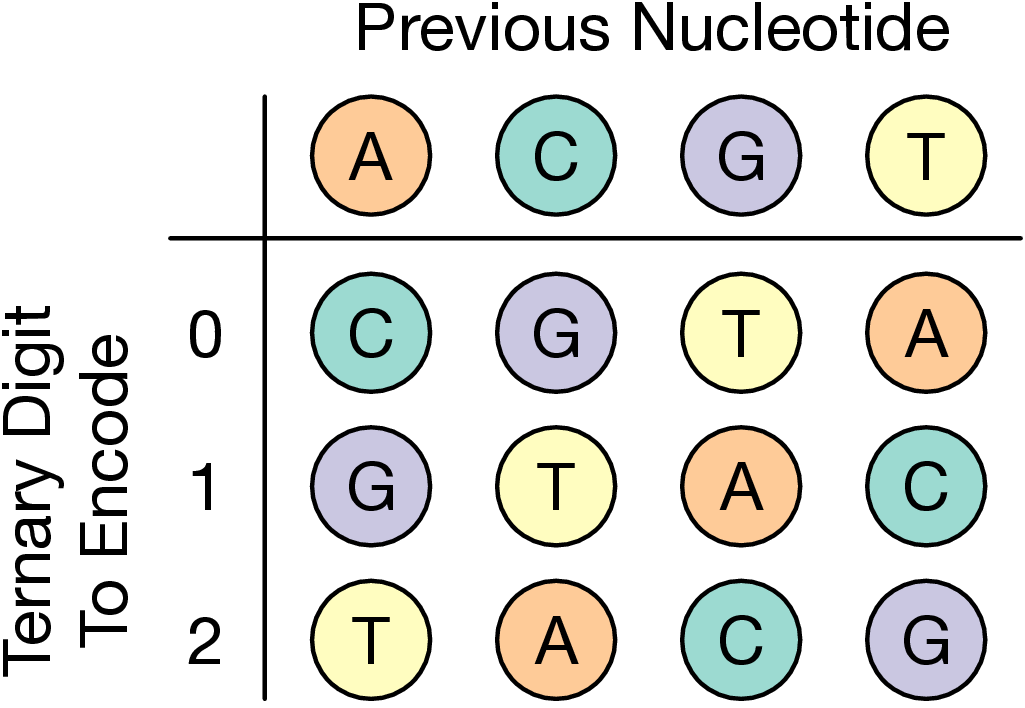
\includegraphics[width=0.5\textwidth]{goldman}
    \caption{Encoding of the trit produced by a 3-ary Huffman tree for each symbol}
    \label{fig:goldman}
\end{figure}

In 2013, Goldman and al. \cite{bib:goldman} proposed an algorithm to encode digital data into binary while respecting the main constraint of DNA sequencing, homopolymers. 
The technique proposes to encode data first in a 3-ary Huffman tree so that each byte can be encoded into the digits $0,1,2$ giving a smaller representation to more frequent data and longer one to less frequent data. 
Once each byte has its own code representation in the tree, the digits can be encoded by mapping to one of the nucleotides while ensuring that the previous encoded nucleotides is not use to encode the current digit. A representation is shown on the Figure~\ref{fig:goldman} for the mapping of the digits regarding the last encoded nucleotide.

\subsection{PAIRCODE}

PAIRCODE \cite{bib:paircode} is a technique proposed in $2019$ to encode any symbols (it is not restricted to binary data) to fixed length codewords.
The quaternary constrained codeword $\mathcal{C}*$ is constructed using mainly pair-elements from the following dictionary:
$$
\mathcal{C}_1=\{AT,AC,AG,TA,TC,TG,CA,CT,GA,GT\}
$$

It is possible to build any codeword of even length by concatening words from these $10$ elements. To build codeword of odd length, it is possible to concatenate one of the word from the dictionary:
$$
\mathcal{C}_2=\{A,C,G,T\}
$$

This construction guarantees that the final encoded DNA stream does not contain homopylmers and a GC-percentage higher than the AT-percentage.



\subsection{JPEG DNA codec}
\label{subsec:jpegdna}

\begin{figure}
    \centering
    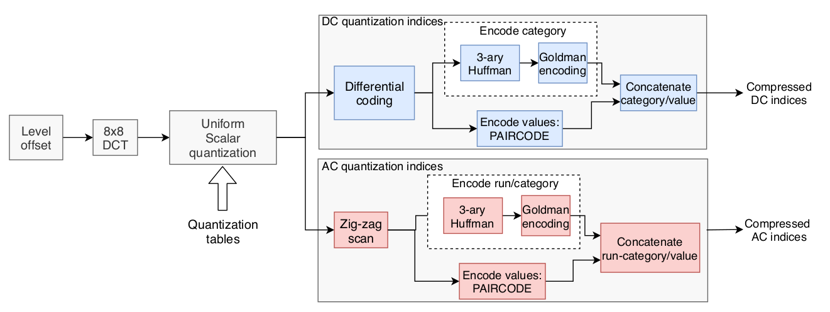
\includegraphics[width=0.7\textwidth]{jpegdna/schema}
    \caption{Schema of the JPEG DNA codec}
    \label{fig:jpegdna}
\end{figure}

The purpose of the JPEG DNA codec is to encode a raw image to DNA code using the JPEG codec and encoding the coefficients to actual DNA nucleotides thanks to the PAIRCODE and Goldman coding.

Before turning an image into a DNA stream, the first steps are to extract the DCT coefficients that are going to be encoded. 

With a raw image as input of shape either H$\times$W (gray image) or H$\times$W$\times$3 (RGB image), the first step is to shift the values of the image by $-128$ to center it around $0$ since the values of the pixels are encoded on \textit{uint8} values and are thus betweem $0$ and $255$. Then the discrete cosine transform is applied on these centered values to extract the ($8\times8$) block DCT coefficients. Next, since the codec is dealing with visual information, a uniform scalar quantization is used to turn continuous values to discrete coefficients thanks to predefined quantization tables that give more importance to low frequency cosines (because the human eye is more sensitive to low frequency signals than high frequency ones).  The quantization introduced a lot of zero for high frequencies on the lower right part of the block. The last step is then to flatten the block DCT quantized coefficients in a zigzag maneer starting from the upper left corner, this way, there will be a large part of zeros at the end of the $64$-long flatten array. 

The flatten array is now composed of the DC value (constant intensity) as first element and then 63 AC values corresponding to each particular cosine frequency. As we will see, the DC and AC values are encoded into DNA in two different ways.


In the classical JPEG workflow, each category is mapped to a binary representation thanks to the Huffman tree that will encode the most frequent AC/DC categories to the shortest words. 
For the DNA version, they used a 3-ary Huffman tree to transform the category into trits and then encode these categories with the Goldman algorithm, the category are determined by the range in which the value falls.
The AC and DC indices are then encoded using a fixed length $l$ codebook that belongs to a code which has been generated using PAIRCODE.

For example, here is how the absolute AC values are categorized:

\begin{minipage}[t]{0.45\textwidth}
\begin{itemize}
    \item $\{0\} \rightarrow 0$
    \item $[1,5] \rightarrow 1$
    \item $[6,17] \rightarrow 2$
    \item $[8,82] \rightarrow 3$
\end{itemize}
\end{minipage}
\begin{minipage}[t]{0.45\textwidth}
\begin{itemize}
    \item $[83,375] \rightarrow 4$
    \item $[376,1263] \rightarrow 5$
    \item $[1264,5262] \rightarrow 6$
    \item $[5263,17579] \rightarrow 7$
\end{itemize}
\end{minipage}

And for each category, we have a fixed number of codewords with fixed length in a specific codebook. Here is the example of the codebooks used in the JPEG DNA codec algorithm per category (as shown on Figure~\ref{fig:codebooks}):

\newpage
\begin{minipage}[t]{0.45\textwidth}
\begin{itemize}
        \item $0 \rightarrow 10$ words of length $2$ 
        \item $1 \rightarrow 24$ words of length $3$
        \item $2 \rightarrow 130$ words of length $4$
        \item $3 \rightarrow 586$ words of length $5$
\end{itemize}
\end{minipage}
\begin{minipage}[t]{0.45\textwidth}
\begin{itemize}
        \item $4 \rightarrow 1776$ words of length $6$
        \item $5 \rightarrow 7998$ words of length $7$
        \item $6 \rightarrow 24634$ words of length $8$
        \item $7 \rightarrow 110660$ words of length $9$
\end{itemize}
\end{minipage}

%    \begin{lstlisting}[language=python]
%def find_category_ac(value):
%    """Find the category of an ac value
%
%    :param value: Value for which we want the category
%    :type value: int
%    :return: Category corresponding to the value
%    :rtype: int
%    """
%    if value == 0:
%        return 0
%    if 1 <= abs(value) <= 5:
%        return 1
%    if 6 <= abs(value) <= 17:
%        return 2
%    if 18 <= abs(value) <= 82:
%        return 3
%    if 83 <= abs(value) <= 375:
%        return 4
%    if 376 <= abs(value) <= 1263:
%        return 5
%    if 1264 <= abs(value) <= 5262:
%        return 6
%    if 5263 <= abs(value) <= 17579:
%        return 7
%    return -1
%    \end{lstlisting}
